% Chapter Template

\chapter{Results} % Main chapter title

\label{Chapter 5} % Change X to a consecutive number; for referencing this chapter elsewhere, use \ref{ChapterX}

\lhead{Chapter 5. \emph{Results}} % Change X to a consecutive number; this is for the header on each page - perhaps a shortened title


\section{ Simulation reproductability}
    
    A large part of implementing a reliable simulation environment is to solve incoherences that can be problematic when used in a learning environment. Many parameters are to be set so that these "bugs" become a minor issue. These incoherences have two different sources : the float approximation, and the approximation of continuous phenomena with time steps. For instance when setting the parameters of a PID loop, the frequency of the loop is a crucial parameter : if it is two low, then the control can become unstable, and in a simulation it cannot be higher than the frequency of the simulation itself. Another example is the fact that collision are not continuous phenomena : in a simulation an object released to fall on the ground will be above the ground for one time step and "inside" the ground at the time step. Physics simulation engines like ODE implement tricks to solve this problem, however with this phenomena and the limited float precision, we can understand that we see a chaotic behavior : two estimations of the same parameters under the same initial condition can lead to different results and therefore two different estimations of the fitness function $f$. Therefore a large part of this project was to reduce the variance of the results of the fitness function on the same parameters for different trials. The graph hereunder present these results with two different settings of the PID frequency.


\begin{figure}[htbp]
    \centering
    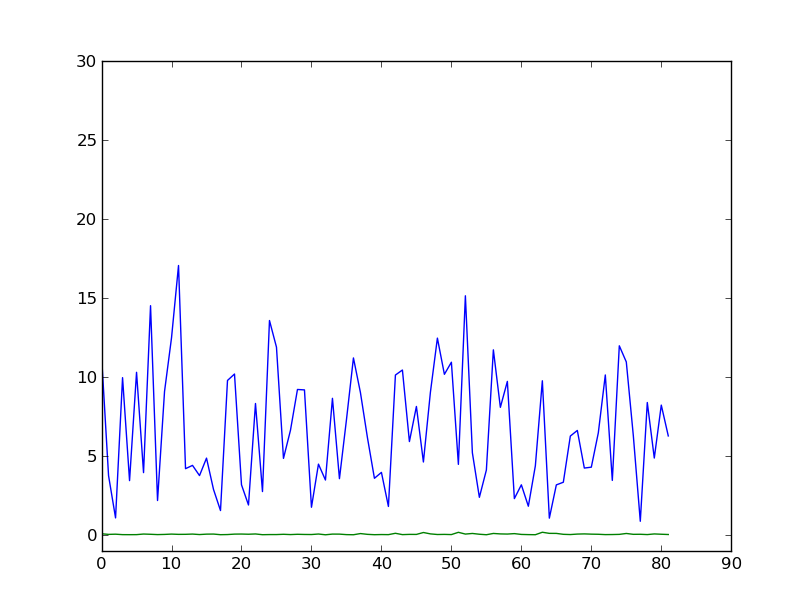
\includegraphics[scale=0.8]{Figures/figure_simulation_consitency.png}
    \rule{35em}{0.5pt}
    \caption[Simulation Consistency]{Variation of fitness function for a PID frequency of 30Hz(Blue) and 100Hz(Green)}
    \label{fig:figure_simulation_consistency}
\end{figure}


    
\section{ Creatures taking advantages of simulation bugs}
Another surprising behavior in the simulation is the fact that the learning algorithm can take advantage of some of the existing bugs in the simulation. This results was also obeserved by Karl Sims \cite{karl}. In the simulation when reinitializing the creature in its starting position, the velocity and position where reinitialized to the starting situation.The problem is that using the approximation of ODE for collision using, some hidden parameters in the simulation were not reinitialized when moving the creature back to its starting position. Therefore, the creature could have some of its blocks under the ground, and was jumping in a really unreallistic way because of this bug. The learning algorithm learned to find the bug and all the best solution were using this bug to jump very far and have a high value for the fitness function.
    
\section { Comparaison }

This section present different curves obtained for the different learning method and learning model. In each graph, the we present the evolution of the evaluation of the fitness function which is the distance that a four-legged creature has walked during the learning period.


\begin{figure}[htbp]
    \centering
    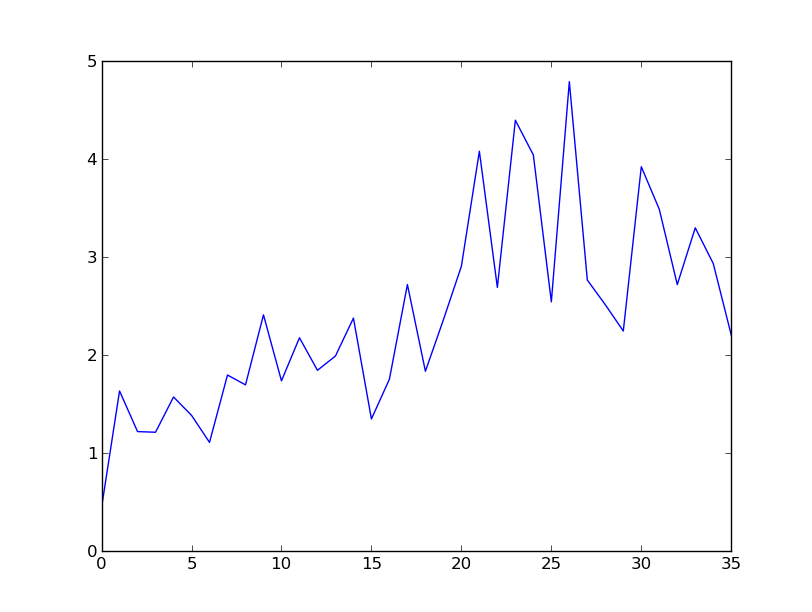
\includegraphics[scale=0.5]{Figures/simplex_fourier.png}
    \rule{35em}{0.5pt}
    \caption[Learning Method : Simplex, Model : Fourier Decomposition]{Learning Method : Simplex, Model : Fourier Decomposition}
    \label{fig:simplex_fourier}
\end{figure}


\begin{figure}[htbp]
    \centering
    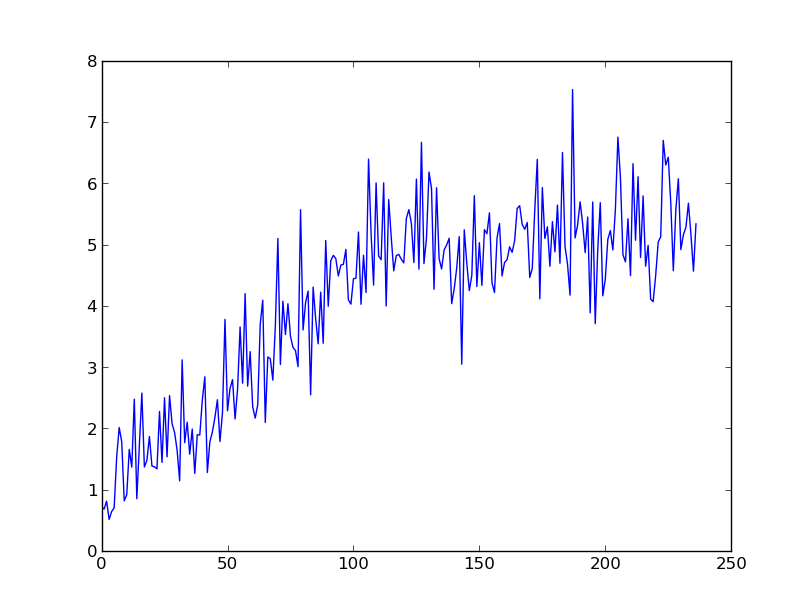
\includegraphics[scale=0.5]{Figures/gen_fourier.png}
    \rule{35em}{0.5pt}
    \caption[Learning Method : GA, Model : Fourier Decomposition]{Learning Method : Genetic Algorithm, Model : Fourier Decomposition}
    \label{fig:simplex_fourier}
\end{figure}

\begin{figure}[htbp]
    \centering
    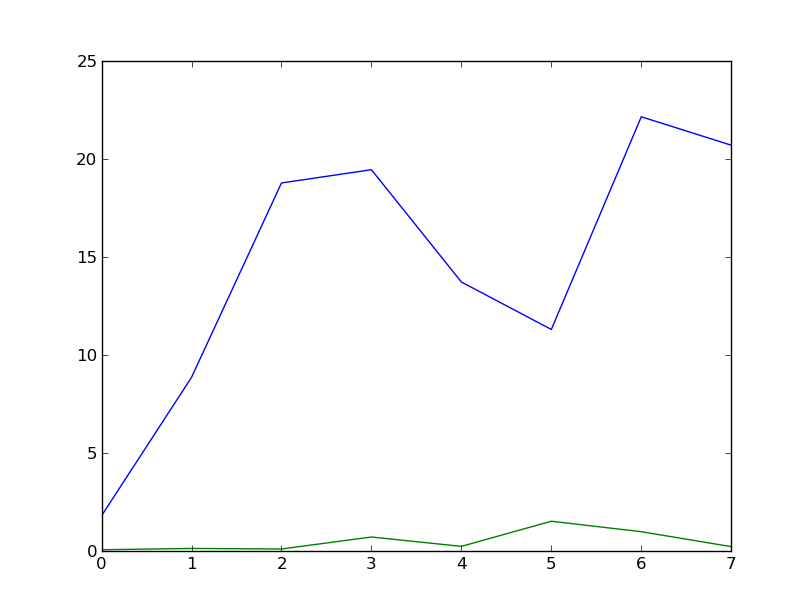
\includegraphics[scale=0.5]{Figures/cpg_simplex.png}
    \rule{35em}{0.5pt}
    \caption[Learning Method : GA, Model : CPG]{Learning Method : Genetic Algorithm, Model : CPG}
    \label{fig:cpg_gen}
\end{figure}


\begin{figure}[htbp]
    \centering
    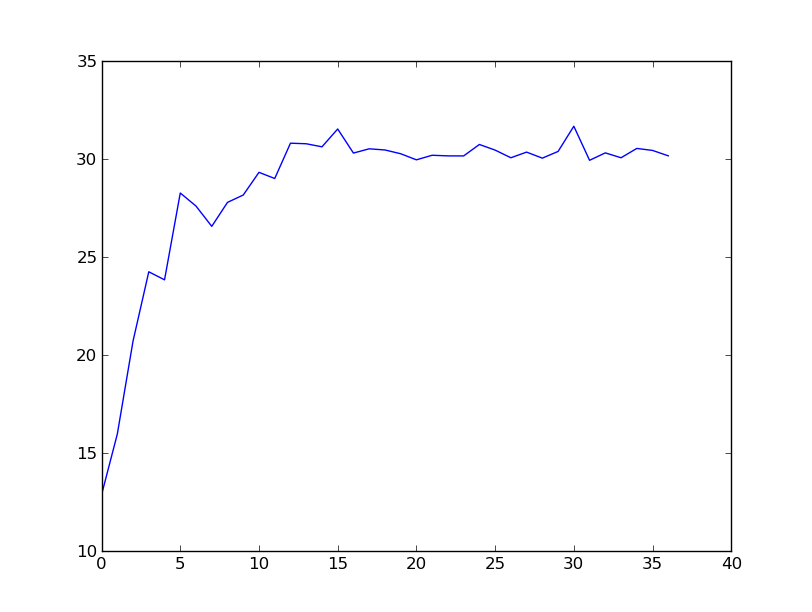
\includegraphics[scale=0.5]{Figures/cpg_gen.png}
    \rule{35em}{0.5pt}
    \caption[Learning Method : GA, Model : CPG]{Learning Method : Genetic Algorithm, Model : CPG}
    \label{fig:cpg_gen}
\end{figure}

\begin{figure}[htbp]
    \centering
    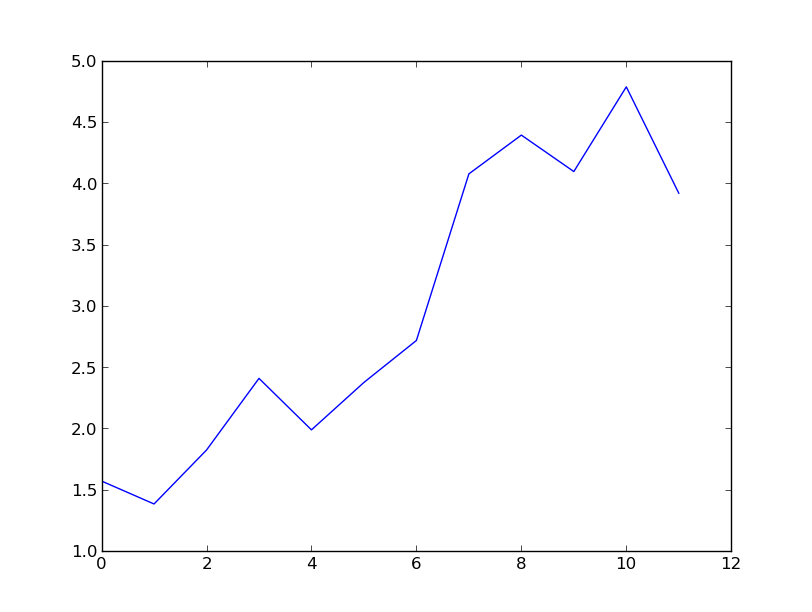
\includegraphics[scale=0.5]{Figures/esn_simplex.png}
    \rule{35em}{0.5pt}
    \caption[Learning Method : Simplex, Model : LMS]{Learning Method : Simplex, Model : Liquid State Machine}
    \label{fig:esn_simplex}
\end{figure}

\begin{figure}[htbp]
    \centering
    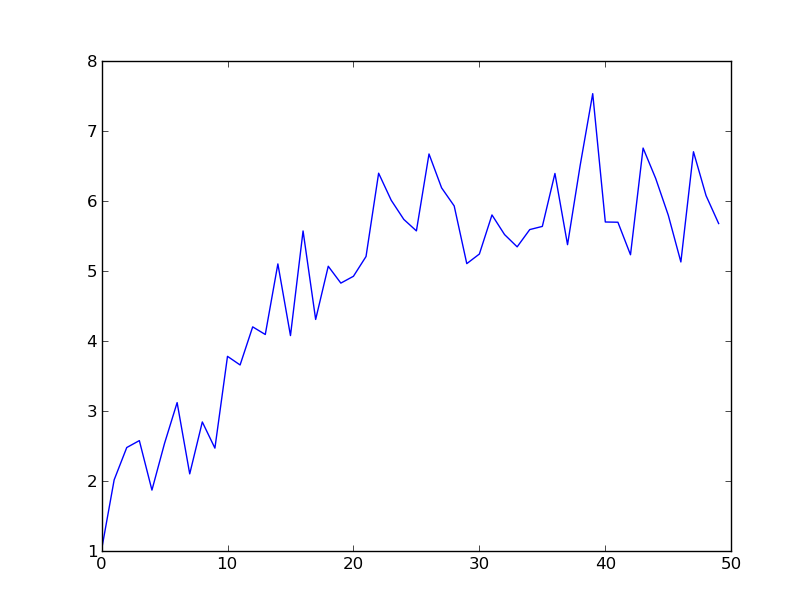
\includegraphics[scale=0.5]{Figures/esn_gen.png}
    \rule{35em}{0.5pt}
    \caption[Learning Method : GA, Model : Liquid State Machine]{Learning Method : Genetic Algorithm, Model : Liquid State Machine}
    \label{fig:esn_gen}
\end{figure}


One of the feature that we can observe in compairing the genetic algorithm and the Nelder Mead method over the different models, is that the genetic algorithm is slower, however it converge towards a higher value. This is an expected behavior as the simplex is a downhill method and therefore converge towards a local minima. One of the example of the convergence of the Nelder-Mead method towards a local extrema that was encountered was a situation where the creature seems to have learn how to push on one leg only to move. 

The best results have been obtained using the CPG and the Genetic Algorithm (see learning curves). In their architecture, central pattern generator follow the physical shape of the creature, where the fourier decomposition and the liquid state machine models are independant of it. Therefore, it is easier to train such a model, because it requires less parameters to produce the angles functions. However we could expect to have better results after a long training for the fourier decomposition and the liquid state machine as well as they are more general models but it is not the case in these results : the learning algorithms are stuck in local minima for these models.



% In the second part of the project, my focus will be on improving the learning algorithms to lead to better solutions. One of the main problem of the movements of these structures is that it optimizes a given paramter (speed, distance with a certain amount of energy, rotation velocity...) but it does not give any control on the structure. In Modular and Swarm Robotics, if we want to make use of such creatures, we need to be able to interact with them, to modify their behaviour. To do so, I want to focus my work on building models to represent how these robots will interact with the world and the orders they receive. Recent deep learning techniques are made possible with the growing accessible computation power and they showed good results on complex problems such as Computer Vision or Sound Recognition. Some of these techniques are good candidate in order to generate complex pattern to understand the structure, generate oscillation for the direct control of joints (Echo State Networks for instance \cite{jaeger2007echo}) and lead to the concept of self-awareness of the mechanical structure of a robot. 

